% Appendix A

\chapter{Appendix}



\section{Appendix}

Network configuration in Virtual machine demo0.

\begin{figure}[bth]
{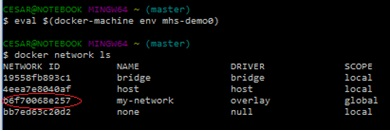
\includegraphics[width=1\linewidth]{gfx/demo0}}\caption[demo0]{demo0}
\label{fig:demo0}
\end{figure}

Network configuration in Virtual machine demo1

\begin{figure}[bth]
{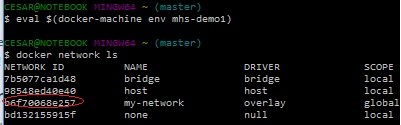
\includegraphics[width=0.7\linewidth]{gfx/demo1}}\caption[demo1]{demo1}
\label{fig:demo1}
\end{figure}
\\

Docker compose with the compute container.
\begin{figure}[bth]
{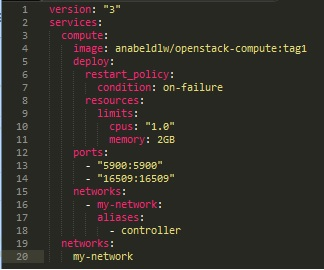
\includegraphics[width=0.6\linewidth]{gfx/compose}}\caption[Docker-compose.yml]{Docker-compose.yml1}
\label{fig:compose}
\end{figure}\\

\\
Criu steps for the correct installation\\

After the installation of the components mentioned in section 6.3, I proceeded to add protobuf in the next way

\begin{lstlisting}[language=bash,frame=tb,caption={Protoc}] 
wget https://github.com/google/protobuf/releases/download/v2.6.0/protobuf-2.6.0.tar.bz2
./configure
make
make check
sudo make install
protoc --version
Protocol buffer version 2.5.0 is installed on your box.
ldconfig
\end{lstlisting}\\

Note: Sometimes the latest version of protocol does not load up. So we can do it manually by ldconfig, other versions of libprotoc must be deleted, and a new container with criu must be installed, in the next way:

\begin{figure}[bth]
{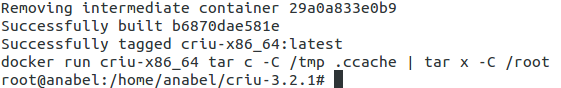
\includegraphics[width=1\linewidth]{gfx/criu}}\caption[Criu]{Criu}
\label{fig:criu}
\end{figure}\\